% questions.tex —— 1965 年·全国卷 · 题目内容片段（无答案）
% 由 tools/generate_projects.py 依来源总账自 1965/1965_数学真题_试题.md 生成，勿手改（改源 MD 后重跑）


\begin{gktip}
\textbf{来源说明}：本题面依据固定源 PDF《1965 年试题》第 1—3 页逐题转录。原卷第 8 题标为“附加题”，不计入正式 7 题题量，单独保留在第 7 题之后。
\end{gktip}

\par\medskip

\Needspace{0.4\textheight}
\begin{question}
\gkti{1}右面的二视图所表示的立体是什么？求出它的体积。图中底面正六边形的边长为 $a$，侧棱长为 $2a$。
\nopagebreak[4]
\begin{center}\begin{tikzpicture}[scale=0.9,>=Stealth]
  % 正视图：正六棱锥的侧棱长标为 2a
  \coordinate (V) at (2.8,3.6);
  \coordinate (L) at (0.3,0.5);
  \coordinate (R) at (5.3,0.5);
  \coordinate (M1) at (1.65,0.5);
  \coordinate (M2) at (3.95,0.5);
  \draw[thick] (L) -- (R) -- (V) -- cycle;
  \draw (V) -- (M1) (V) -- (M2);
  \draw[<->] (0.62,0.78) -- (2.63,3.28) node[midway,left] {$2a$};
  \node[below] at (2.8,0.25) {正视图};

  % 俯视图：正六边形边长为 a
  \coordinate (O) at (2.8,-1.45);
  \coordinate (H1) at (1.0,-1.45);
  \coordinate (H2) at (1.9,-0.0);
  \coordinate (H3) at (3.7,-0.0);
  \coordinate (H4) at (4.6,-1.45);
  \coordinate (H5) at (3.7,-2.9);
  \coordinate (H6) at (1.9,-2.9);
  \draw (H1) -- (H2) -- (H3) -- (H4) -- (H5) -- (H6) -- cycle;
  \draw (O) -- (H1) (O) -- (H2) (O) -- (H3)
    (O) -- (H4) (O) -- (H5) (O) -- (H6);
  \draw[<->] (1.95,-2.72) -- (3.65,-2.72) node[midway,below] {$a$};
  \node[below] at (2.8,-3.18) {俯视图};
\end{tikzpicture}
\end{center}
\nopagebreak[4]
\Needspace{0.4\textheight}
\end{question}
\begin{question}
\gkti{2}在 $A$ 处的甲船测得乙船在北偏西 $49^\circ48'$ 的 $B$ 处，以速度 $22$ 浬/小时向正北方向行驶。甲船立即从 $A$ 处出发，以速度 $26$ 浬/小时向北偏西 $a$ 度的方向沿直线驶去，追赶乙船。问 $a$ 是多大角度时，经过一段时间，甲船能够在某处 $C$ 恰好与乙船相遇？（$\lg2.2=0.3424$，$\lg2.6=0.4150$；$\lg$ 是以 $10$ 为底的对数符号。）
\nopagebreak[4]
\begin{center}\begin{tikzpicture}[scale=0.9,>=Stealth]
  \coordinate (A) at (0,0);
  \coordinate (B) at (-1.25,1.25);
  \coordinate (C) at (-0.72,2.75);
  \draw[->] (0,-0.55) -- (0,3.45) node[above] {北};
  \draw[->] (-2.2,0) -- (2.25,0) node[right] {东};
  \node[left] at (-2.2,0) {西};
  \node[below] at (0,-0.55) {南};
  \draw[thick] (A) -- (B) -- (C);
  \draw[thick,dashed] (A) -- (C);
  \fill (A) circle (1.4pt) node[below right] {$A$};
  \fill (B) circle (1.4pt) node[left] {$B$};
  \fill (C) circle (1.4pt) node[above left] {$C$};
  \node at (-0.95,0.82) {$49^\circ48'$};
  \node at (-0.36,1.58) {$a$};
  \node[below right] at (0.15,1.6) {甲船航向};
  \node[right] at (-0.55,2.25) {乙船向北};
\end{tikzpicture}
\end{center}
\nopagebreak[4]
\begin{gktip}
原卷附有正弦、余弦对数表；本题计算直接用到的正弦对数表值为：$\lg\sin49^\circ48'=1.8830$，查表 $\lg\sin40^\circ15'=1.8104$。
\end{gktip}

\Needspace{0.4\textheight}
\end{question}
\begin{question}
\gkti{3}把地球看作半径为 $R$ 的球。设 $A$、$B$ 两地的纬度相同，都是 $a$ 度，它们的经度相差 $\beta$ 度（$0^\circ<\beta\leqslant180^\circ$）。求 $A$、$B$ 两地之间的球面距离（即大圆弧长）。
\nopagebreak[4]
\begin{center}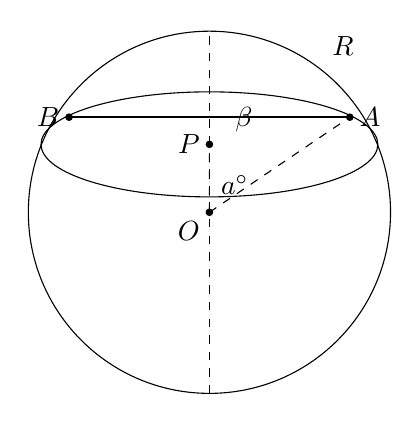
\begin{tikzpicture}[scale=1.15]
  \draw (0,0) circle (2);
  \draw[dashed] (0,-2) -- (0,2);
  \draw (0,0.75) ellipse (1.86 and 0.58);
  \coordinate (O) at (0,0);
  \coordinate (P) at (0,0.75);
  \coordinate (A) at (1.55,1.05);
  \coordinate (B) at (-1.55,1.05);
  \draw[thick] (A) -- (B);
  \draw[dashed] (O) -- (A) (O) -- (P);
  \fill (O) circle (1.2pt) node[below left] {$O$};
  \fill (P) circle (1.2pt) node[left] {$P$};
  \fill (A) circle (1.2pt) node[right] {$A$};
  \fill (B) circle (1.2pt) node[left] {$B$};
  \node at (0.38,1.02) {$\beta$};
  \node at (0.28,0.30) {$a^\circ$};
  \node[above right] at (1.25,1.62) {$R$};
\end{tikzpicture}
\end{center}
\nopagebreak[4]
\end{question}
\begin{question}
\gkti{4}

（1） 证明 $|\sin2x|\leqslant2|\sin x|$。（$x$ 为任意值。）

（2） 已知 $n$ 为任意正整数，用数学归纳法证明 $|\sin nx|\leqslant n|\sin x|$。（$x$ 为任意值。）

\Needspace{0.4\textheight}
\end{question}
\begin{question}
\gkti{5}已知一点 $P$ 的坐标是 $(4,-2)$，直线 $l$ 的方程是 $y-x+5=0$，曲线 $C$ 的方程是

\nopagebreak[4]
\[\frac{(x+1)^2}{2}+\frac{(y-1)^2}{4}=1.\]

求经过 $P$ 点而与 $l$ 垂直的直线和曲线 $C$ 的交点坐标，并画出此题的略图。
\nopagebreak[4]
\begin{center}\begin{tikzpicture}[scale=0.9,>=Stealth]
  \draw[->] (-3.0,0) -- (3.8,0) node[right] {$x$};
  \draw[->] (0,-3.0) -- (0,3.3) node[above] {$y$};
  \draw (0,0) ellipse (1.45 and 2.15);
  \draw[thick] (-2.2,2.2) -- (3.2,-3.2);
  \coordinate (I1) at (0.48,1.72);
  \coordinate (I2) at (-1.05,3.0);
  \fill (I1) circle (1.3pt) node[right] {$\left(\frac13,\frac53\right)$};
  \fill (I2) circle (1.3pt) node[above left] {$(-1,3)$};
  \fill (2.6,-2.6) circle (1.3pt) node[below right] {$P(4,-2)$};
  \node[below left] at (0,0) {$O$};
  \node at (1.75,1.35) {$C$};
\end{tikzpicture}
\end{center}
\nopagebreak[4]
\end{question}
\begin{question}
\gkti{6}当 $p$ 是什么实数时，方程 $x^2+px-3=0$ 与方程 $x^2-4x-(p-1)=0$ 有一个公共根？并求出这个公共根。

\Needspace{0.4\textheight}
\end{question}
\begin{question}
\gkti{7}已给抛物线 $y^2=2x$。

\Needspace{5\baselineskip}
（1） 在抛物线上任取两点 $P_1(x_1,y_1)$、$P_2(x_2,y_2)$。经过线段 $P_1P_2$ 的中点作直线平行于抛物线的轴，和抛物线交于点 $P_3$。证明

\nopagebreak[4]
\[\triangle P_1P_2P_3\text{ \text{的面积}}=\frac1{16}|y_1-y_2|^3.\]

（2） 经过线段 $P_1P_3$ 和 $P_2P_3$ 的中点，分别作直线平行于抛物线的轴，和抛物线依次交于 $Q_1$、$Q_2$。试将 $\triangle P_1P_3Q_1$ 与 $\triangle P_2P_3Q_2$ 的面积的和用 $y_1$、$y_2$ 表示出来。

（3） 仿照（2），又可以作出四个更小的三角形。照这样继续下去，可以作出一系列的三角形。由此设法求出线段 $P_1P_2$ 与抛物线所围成的图形的面积。
\nopagebreak[4]
\begin{center}\begin{tikzpicture}[scale=0.9,>=Stealth]
  \draw[->] (-0.35,0) -- (4.5,0) node[right] {$x$};
  \draw[->] (0,-2.35) -- (0,2.35) node[above] {$y$};
  \draw[domain=-2.1:2.1,smooth,variable=\t,thick]
    plot ({0.5*\t*\t},{\t});
  \coordinate (P1) at (3.2,1.7);
  \coordinate (P2) at (2.6,-1.55);
  \coordinate (P3) at (0.22,0.08);
  \coordinate (Q1) at (0.92,0.89);
  \coordinate (Q2) at (0.72,-0.74);
  \draw[thick] (P1) -- (P2) -- (P3) -- cycle;
  \draw[thick] (P1) -- (Q1) -- (P3);
  \draw[thick] (P2) -- (Q2) -- (P3);
  \draw[dashed] (P3) -- (Q1) (P3) -- (Q2);
  \fill (P1) circle (1.3pt) node[above right] {$P_1$};
  \fill (P2) circle (1.3pt) node[below right] {$P_2$};
  \fill (P3) circle (1.3pt) node[left] {$P_3$};
  \fill (Q1) circle (1.3pt) node[above right] {$Q_1$};
  \fill (Q2) circle (1.3pt) node[below right] {$Q_2$};
\end{tikzpicture}
\end{center}
\nopagebreak[4]
\Needspace{0.25\textheight}
\textbf{附加题}

\Needspace{5\baselineskip}
（1） 已知 $a$、$b$、$c$ 为实数，证明 $a$、$b$、$c$ 都为正数的充要条件是：

\nopagebreak[4]
\[a+b+c>0,\qquad ab+bc+ca>0,\qquad abc>0.\]

\Needspace{5\baselineskip}
（2） 已知方程

\nopagebreak[4]
\[x^3+px^2+qx+r=0\]

\Needspace{5\baselineskip}
的三个根 $\alpha$、$\beta$、$\gamma$ 都是实数，证明 $\alpha$、$\beta$、$\gamma$ 是一个三角形的三个边长的充要条件是

\nopagebreak[4]
\[p<0,\qquad q>0,\qquad r<0,\qquad p^3>4pq-8r.\]

\end{question}